%%=============================================================================
%% Push-notificaties
%%=============================================================================

\chapter{Notificaties}%
\label{ch:notificaties}

In dit hoofdstuk worden de lokale notificaties van native en cross-platform vergeleken met elkaar. 
Met de resultaten kan dan een gepaste conclusie worden gevormd.

\section{Native}
\subsubsection{Wat is er nodig}
Om lokale notificaties aan te kunnen maken bij Android wordt de NotificationCompat API aangeboden 
door de Android support library. Deze stelt ons in staat om de titel, tekst, pictogram en andere inhoud van de 
notificatie in te stellen. Notificaties kunnen ook worden ingesteld om speciale acties te ondernemen bij het openen 
van de applicatie via de notificatie. Er kan ook een eventueel een prioriteit worden meegegeven.

\subsubsection{Uitvoering}

\paragraph{1. Dependancy toevoegen}
Normaal zijn bevatten alle projecten gestart met Android Studio de nodige dependancies om de NotificationCompat API
te gebruiken. Maar voor de zekerheid verifiëren we dat onderstaande dependancy er bij zit.
\begin{minted}{java}
  val core_version = "1.6.0"
  dependencies {
      implementation("androidx.core:core-ktx:$core_version")
  }
\end{minted}
Als de dependancy is toegevoegd dan kunnen we notificaties beginnen aanmaken.

\paragraph{2. Notificatie aanmaken}
Om een notificatie aan te maken gaan we het NotificationCompat.Builder object gebruiken. 
\begin{minted}{kotlin}
  private fun createNotification(title: String, body: String) {
    val builder = NotificationCompat.Builder(this, CHANNEL_ID)
      .setSmallIcon(icon)
      .setContentTitle(title)
      .setContentText(body)
      .setPriority(NotificationCompat.PRIORITY_DEFAULT)

    val notificationManager: NotificationManager =
      getSystemService(Context.NOTIFICATION_SERVICE) as NotificationManager
    notificationManager.notify(notificationId, builder.build())
}
\end{minted}
\begin{figure}[H]
    \centering
    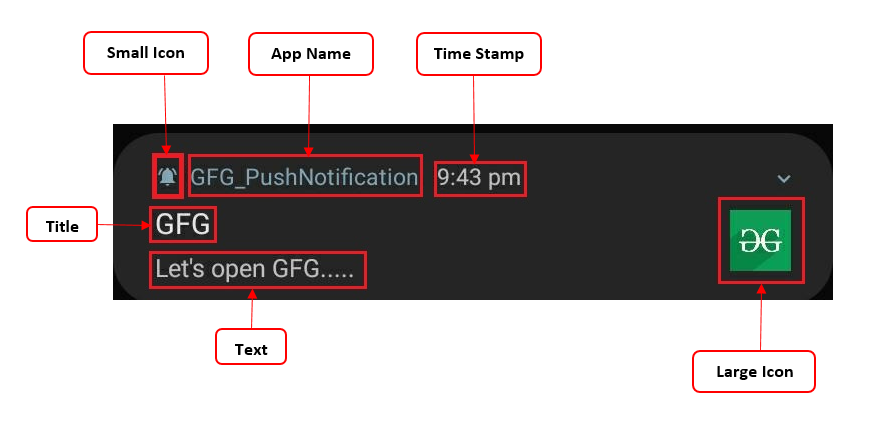
\includegraphics[height=0.3\textheight]{NotificationAnatomy.png}
    \caption{Anatomy standaard notificatie \parencite{One2020}.}
\end{figure}

\paragraph{3. Channel aanmaken}
Het laatste dat we nodig hebben vooraleer de notificatie getoond kan worden is een channel. Deze worden 
gebruikt om notificaties te groeperen volgens hun belang. Om een channel aan te maken gebruiken we 
de .createNotificationChannel() methode. Het maakt niet uit wanneer of waar deze code wordt uitgevoerd. 
Het is enkel belangrijk dat de channel wordt aangemaakt vooraleer er wordt geprobeerd om notificaties 
te tonen. Dus best zo vroeg mogelijk in de applicatie.
\begin{minted}{kotlin}
private fun createNotificationChannel() {
  if (Build.VERSION.SDK_INT >= Build.VERSION_CODES.O) {
    val name = "bachproef"
    val descriptionText = "bachproef notificaties"
    val importance = NotificationManager.IMPORTANCE_DEFAULT
    val channel = NotificationChannel(CHANNEL_ID, name, importance).apply {
      description = descriptionText
    }
    // Channel bij het systeem registreren
    val notificationManager: NotificationManager =
      getSystemService(Context.NOTIFICATION_SERVICE) as NotificationManager
    notificationManager.createNotificationChannel(channel)
  }
}
\end{minted}

\paragraph{4. Applicatie maken}
Met deze informatie kunnen we nu een applicatie opbouwen die notificaties zal sturen. De applicatie bestaat 
uit twee \textbf{EditText} componenten voor een titel en beschijving van de notificatie en tot slot een 
\textbf{Button} om de notificatie te triggeren. Als de knop wordt ingedrukt dan wordt de 
\textbf{createNotification} methode aangeroepen en wordt de waarde van de inputs meegegeven.
\begin{figure}[H]
  \centering
  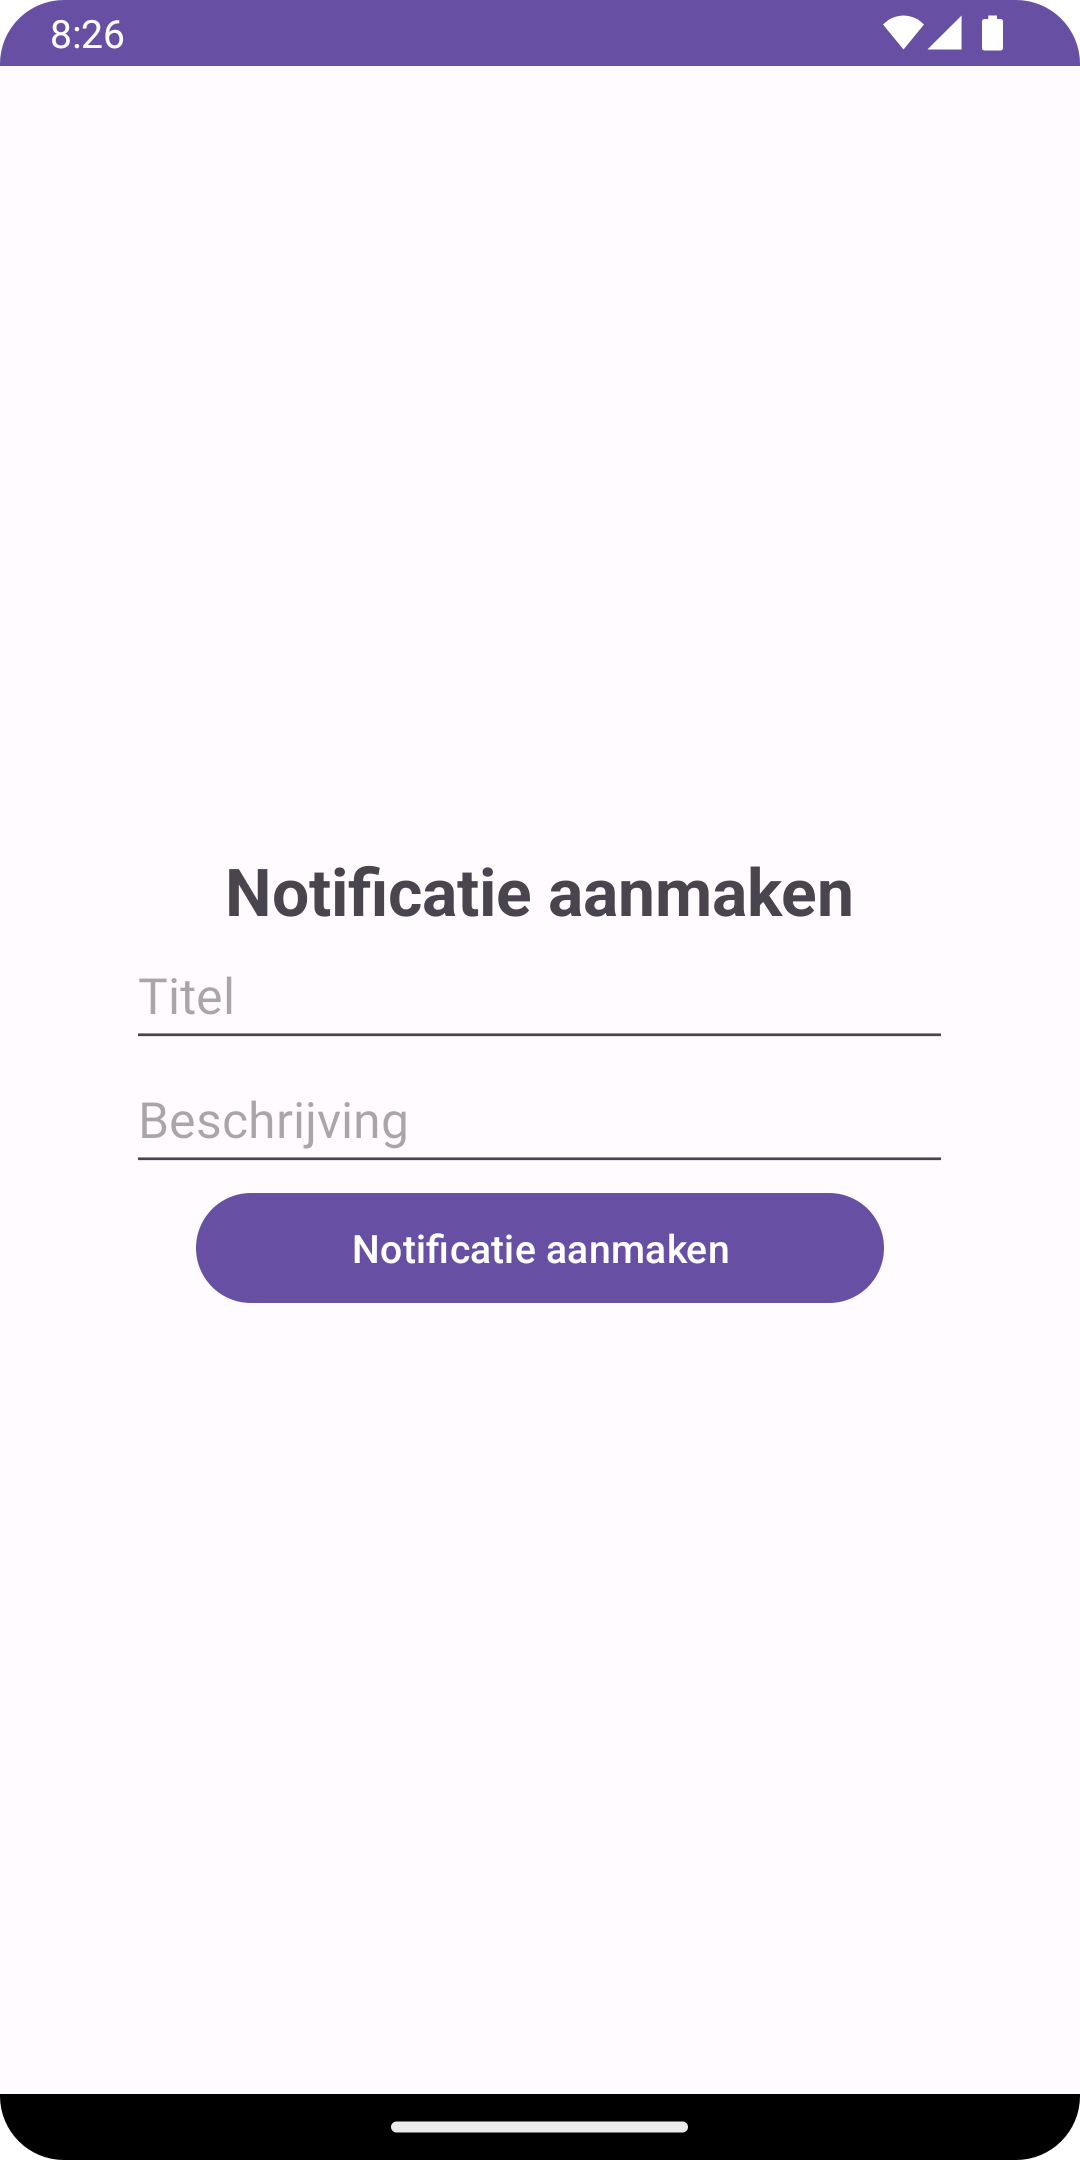
\includegraphics[height=0.5\textheight]{notificaties_layoutnative.png}
  \caption{Layout van applicatie voor notificaties te sturen bij Android.}
\end{figure}

\subsubsection{Ontwikkeltijd}

Ondanks dat er een probleem heeft opgedaan bij het implementeren van de functionaliteit, was 
het implementeren van de notificaties vrij simpel. Als de tijdsduur van het probleem niet wordt meegerekend 
dan kostte het 1 uur en 15 minuten om notificaties te sturen.

\paragraph{Problemen}
Naast de tijd die nodig was om de functionaliteit te implementeren is er ook 2 uur verloren aan een probleem. 
Waarom het probleem zich voordeed is niet duidelijk maar de applicatie vroeg ondanks dat de 
\textbf{POST\_NOTIFICATIONS} bij user-permissions in het AndroidManifest.xml bestand stond 
niet om toestemming om notificaties te sturen. Hierdoor leek het alsof er geen notificaties werden aangemaakt
terwijl het probleem was dat de applicatie geen toestemming had gegeven om notificaties te ontvangen.

\subsubsection{Performantie}

\paragraph{Tijdsduur}
\begin{figure}[H]
    \centering
    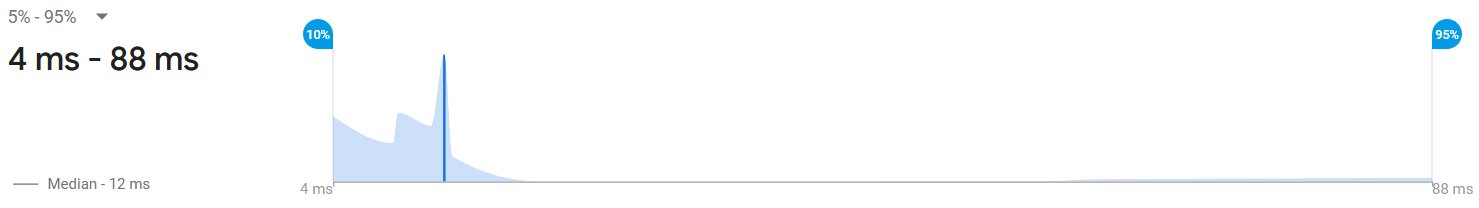
\includegraphics[height=0.1\textheight]{notificatiesDuratieNative.png}
    \caption{Overzicht tijdsduur aanmaken notificaties bij Android.}
\end{figure}
Tijdens het meten van de duur voor het aanmaken van een notificatie, is er 
10 keer een notificatie aangemaakt. Na 10 keer een notificatie aan te maken is er  
een gemiddelde duur van 12ms en met een minimum en 
maximum van 4ms en 88ms.

\paragraph{CPU \& geheugen}
\begin{figure}[H]
    \centering
    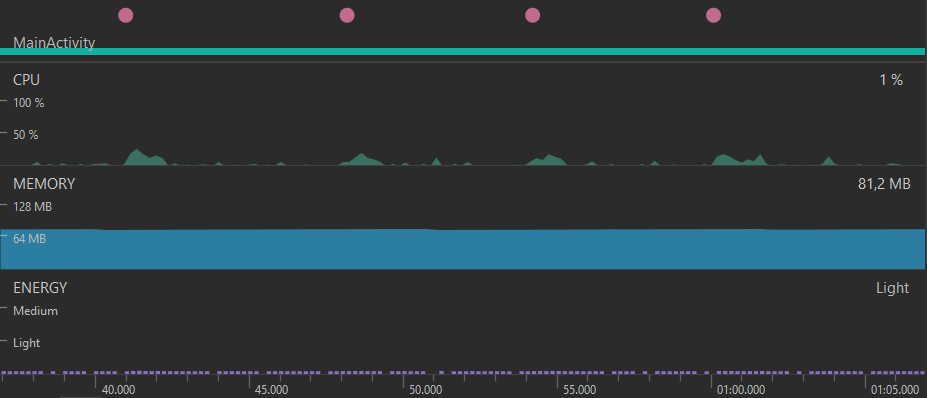
\includegraphics[height=0.25\textheight]{notificatiesPerformantieNative.png}
    \caption{Overzicht CPU en geheugen gebruik tijdens aanmaken notificaties bij Android.}
\end{figure}
Op de grafiek is te zien dat het CPU gebruik van de applicatie wanneer deze inactief is, rond de 4\% ligt. 
Het is ook duidelijk zichtbaar wanneer een notificatie wordt aangemaakt. De piek van het CPU gebruik lag 
gemiddeld op 21\% en schommelde tussen de 19\% en 27\%. Het geheugen blijft in tegenstelling met de CPU 
wanneer de applicatie inactief en actief is, rond de 81MB hangen, met verschillen van maximum 2-3MB. Er is geen 
merkbaar verschil in het geheugen wanneer een notificatie wordt aangemaakt.
  

\subsubsection{Schaalbaarheid}

\paragraph{Complexiteit}
De NotificationCompat API die Android aanbiedt is gemakkelijk om te gebruiken. 
Er moeten normaal gezien geen extra stappen ondernomen worden om de notificaties 
te gebruiken.

\paragraph{Herbruikbaarheid}
het is mogelijk om alle delen van de logica weg te steken in methodes. Op die manier 
is het gemakkelijk om de notificaties later uit te breiden door bijvoorbeeld meerdere channels aan te maken
of op andere plaatsen in het programma een notificatie aan te maken. Het is daardoor ook gemakkelijk om de 
bestaande logica van een notificatie aan te maken te wijzigen aangezien deze allemaal op 1 plaats staan.

\clearpage
\section{Cross-platform}
\subsubsection{Wat is er nodig}
Om lokale notificaties bij React Native te tonen wordt de library Notifee gebruikt.
Deze library geeft ons toegang om net zoals bij Android de titel, tekst, pictogram en 
andere inhoud van de notificatie in te stellen. Daarnaast kunnen er ook speciale acties 
of prioriteiten worden ingesteld.

\subsubsection{Uitvoering}

\paragraph{1. Library toevoegen}
Eerst moet de Notifee library aan de root van ons project worden toegevoegd. 
Deze wordt toegevoegd met volgend commando:
\begin{minted}{bash}
npm install --save @notifee/react-native
\end{minted}

\paragraph{2. Toestemming vragen \& channel aanmaken}
Nog voor een notificatie kan getoond worden, moet er eerst toestemming worden gevraagd. 
Aangezien dit bij React Native niet automatisch gebeurt zoals bij Android moet de 
toestemming programmatisch gevraagd worden. Daarnaast zal ook een channel moeten aangemaakt worden.
Net zoals bij Android maakt het niet uit wanneer dit gebeurt maar het moet wel gebeuren 
voordat er notificaties worden gestuurd. Dus best zo vroeg mogelijk in de applicatie.
\begin{minted}{javascript}
export const notificationsSetup = async () => {
  const PERMISSION = await notifee.requestPermission();

  if(PERMISSION.authorizationStatus === AuthorizationStatus.DENIED) {
    return;
  }

  await notifee.createChannel({
    id: 'bachproef',
    name: 'BachproefNotificaties',
  });
}

\end{minted}

\paragraph{3. Notificatie aanmaken}
Bij React Native worden notificaties direct getoond bij het maken ervan. Net zoals bij Android 
wordt er een naam, description, channelId en optioneel een icoon (default ic\_launcher) meegegeven. 
\begin{minted}{javascript}
export const createNotification = async (title: string, body: string) => {
  await notifee.displayNotification({
    title,
    body,
    android: {
      channelId: 'bachproef',
      pressAction: {
        id: 'default',
      },
    },
  });
}
\end{minted}

\paragraph{4. Applicatie maken}
Net zoals bij native zal de applicatie bestaan 
uit twee \textbf{<TextInput/>} componenten voor een titel en beschijving van de notificatie en tot slot een 
\textbf{<Button/>} om de notificatie te triggeren. Als de knop wordt ingedrukt dan wordt de 
\textbf{createNotification} methode aangeroepen en wordt de waarde van de inputs meegegeven.
\begin{figure}[H]
  \centering
  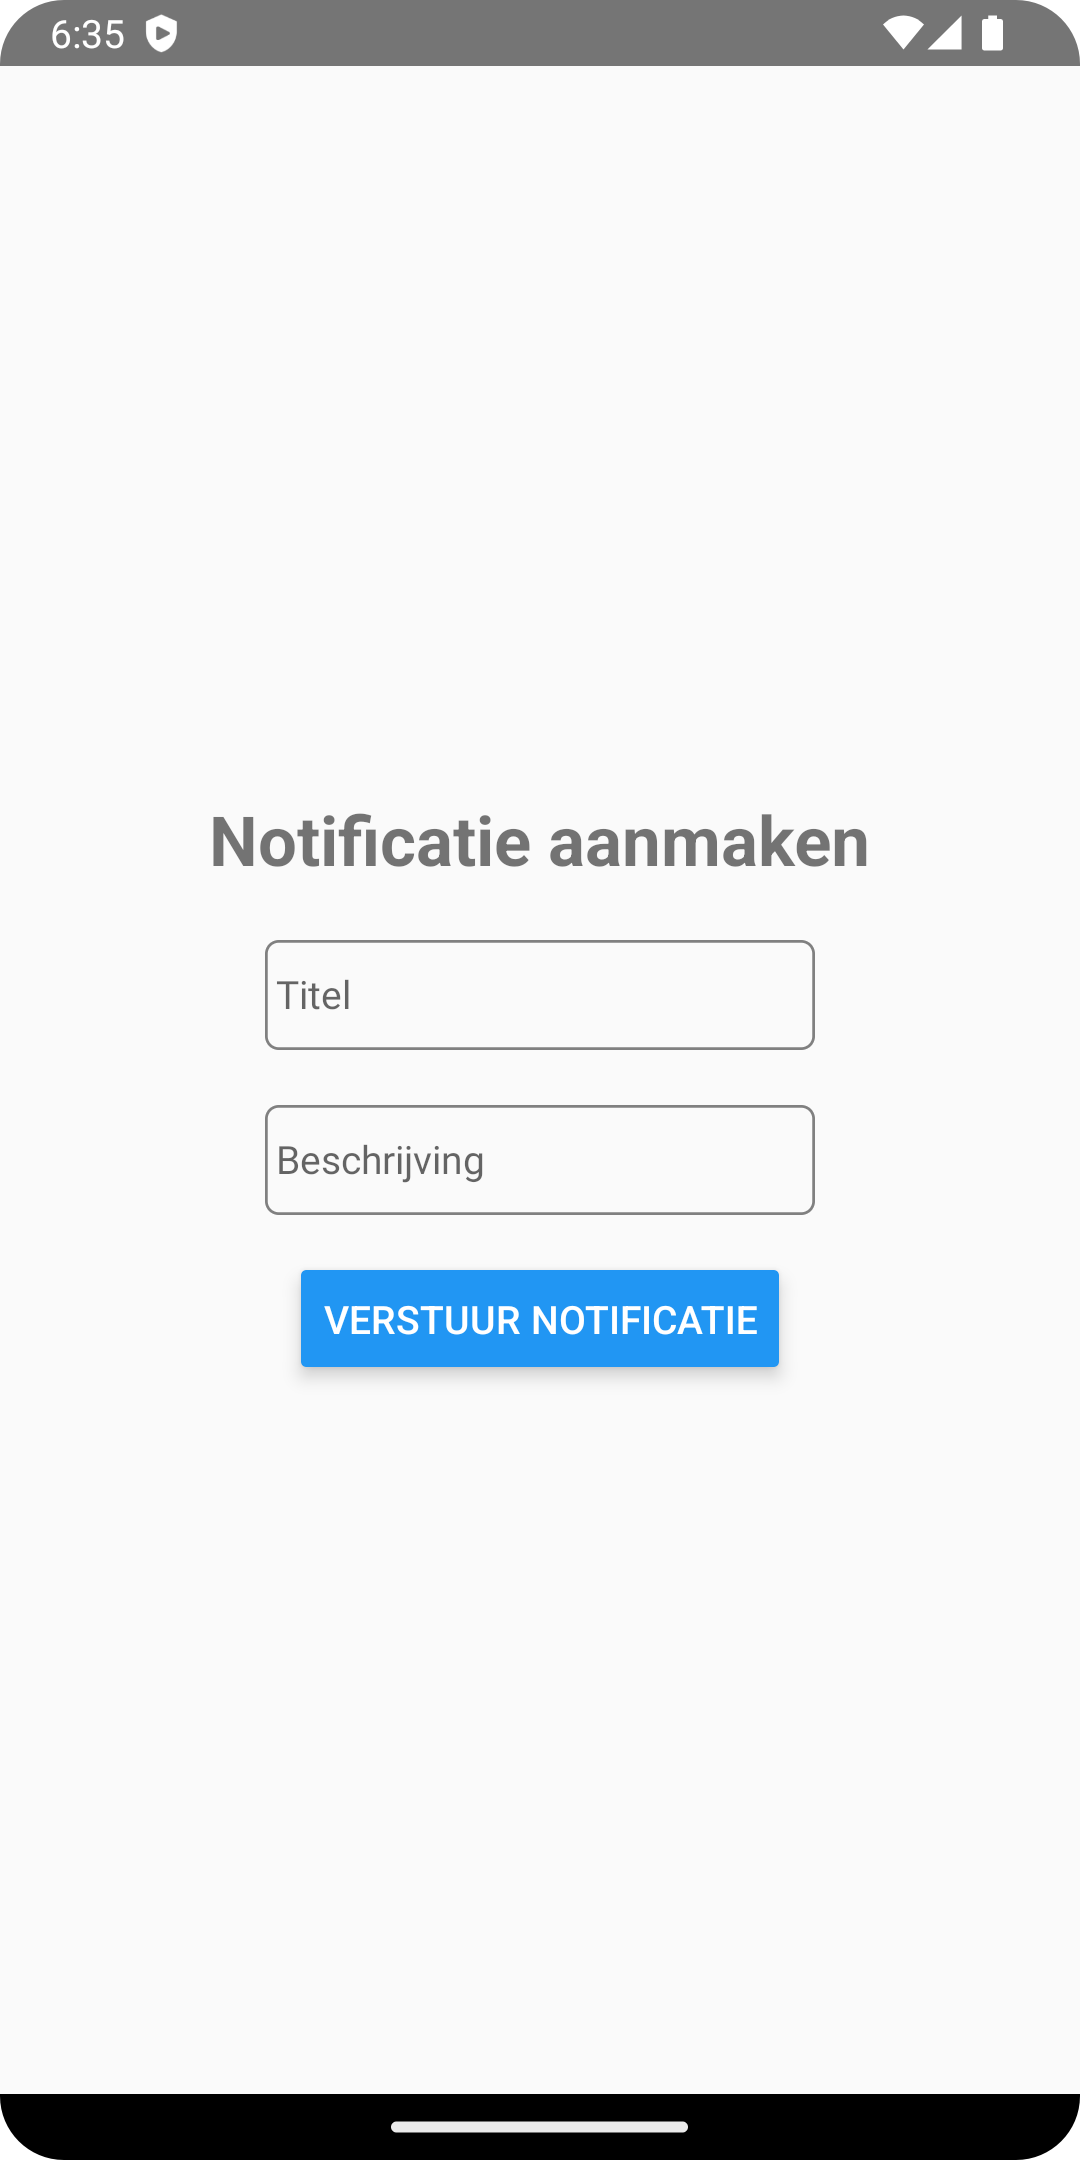
\includegraphics[height=0.5\textheight]{notificaties_layoutcross.png}
  \caption{Layout van applicatie voor notificaties te sturen bij React Native.}
\end{figure}

\subsubsection{Ontwikkeltijd}

Ondanks dat er een externe library gebruikt en geïmplementeerd moest worden, was het implementeren van de 
notificaties functionaliteit zeer simpel. Door gebruik te maken van de documentatie was het mogelijk om 
notificaties te sturen na 1 uur werk. Er zijn ook geen grote problemen of bugs voorgekomen tijdens de implementatie.



\subsubsection{Performantie}

\paragraph{Tijdsduur}
\begin{figure}[H]
  \centering
  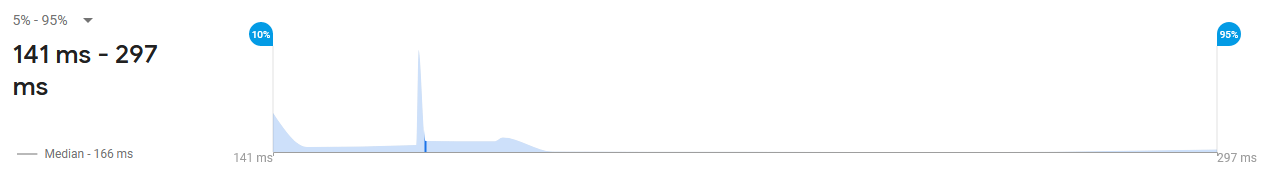
\includegraphics[height=0.085\textheight]{notificatiesDuratieCross.png}
  \caption{Overzicht tijdsduur aanmaken notificaties bij React Native.}
\end{figure}
Tijdens het meten van de duur voor het aanmaken van een notificatie, is er net zoals bij native 
10 keer een notificatie aangemaakt. Na 10 keer een notificatie aan te maken is er 
een gemiddelde duur van 166ms en met een minimum en 
maximum van 141ms en 297ms voor het aanmaken van een notificatie.

\paragraph{CPU \& geheugen}
\begin{figure}[H]
  \centering
  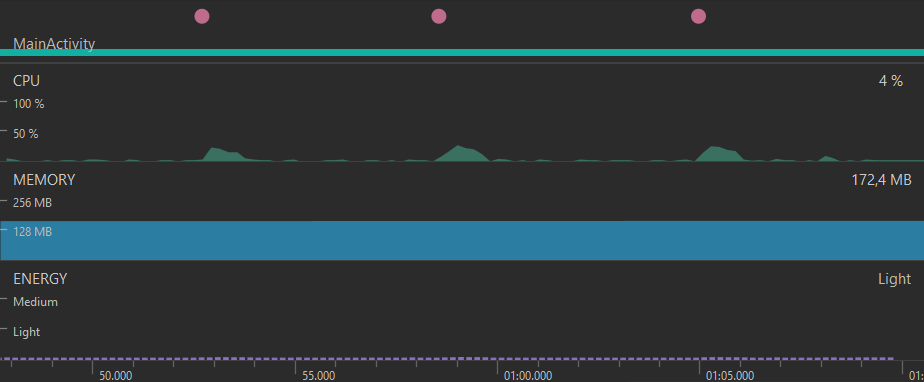
\includegraphics[height=0.25\textheight]{notificatiesPerformantieCross.png}
  \caption{Overzicht CPU en geheugen gebruik tijdens aanmaken notificaties bij React Native.}
\end{figure}
Op de grafiek is te zien dat het CPU gebruik van de applicatie wanneer deze inactief is, rond de 4\% ligt. 
Daarnaast is het duidelijk zichtbaar wanneer een notificatie wordt aangemaakt. De piek van het CPU gebruik lag 
gemiddeld op 28\% en schommelde tussen de 25\% en 30\%. Het geheugen blijft in tegenstelling tot de CPU 
wanneer de applicatie inactief en actief is, rond de 172MB hangen, met verschillen van maximum 0,5MB. 
Er is geen merkbaar verschil in het geheugen wanneer een notificatie wordt aangemaakt.


\subsubsection{Schaalbaarheid}

\paragraph{Complexiteit}
De complexiteit van de library valt goed mee, dankzij de beschikbare documentatie van de library is het zeer 
gemakkelijk om alle mogelijkheden van de library terug te vinden en zelf in een project te implementeren. 

\paragraph{Herbruikbaarheid}
\begin{figure}[H]
    \centering
    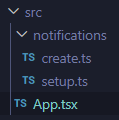
\includegraphics[height=0.1\textheight]{notificationsschaalbaarheidcross.png}
    \caption{Structuur notificaties implementatie React Native.}
\end{figure}
Door de logica van de library op te delen is het gemakkelijk om later opnieuw dezelfde logica op andere plaatsen 
in de code te gebruiken. Er moet enkel een methode geïmporteerd worden om een notificatie aan te maken. Aan die methode 
wordt dan de titel en beschrijving meegegeven. Het is ook mogelijk om de logica voor het aanmaken van een notificatie 
aan te passen. Dit kan dan gemakkelijk gebeuren in het \textbf{create.ts} bestand. Of er kan een nieuwe methode worden 
aangemaakt om bijvoorbeeld de notificatie in te plannen op een later tijdstip.

\section{Conclusie}
Bij de tijdsduur dat nodig is om een notificatie aan te maken is er een duidelijk 
verschil tussen Android en React Native. Gemiddeld is het aanmaken van een notificatie bij Android
154ms sneller dan bij React Native. Bij React Native duurt het gemiddeld 166ms om een notificatie 
aan te maken terwijl dit bij Android maar 12ms duurt. Dit kan liggen aan het feit dat de externe 
library de code moet omzetten naar platformspecifieke code waardoor er veel tijd wordt verloren.
\\\\
Bij het geheugen is er geen verschil tussen het aanmaken van een notificatie en wanneer er 
niks gebeurd in de appplicatie. Desondanks dat er geen invloed is bij het aanmaken van een notificatie 
Gebruikt React Native 112,35\% meer geheugen dan Android (81MB in vergelijking met 172MB). 
Dit kan opnieuw liggen aan het feit dat de externe library
de code moet omzetten naar platformspecifieke code waardoor er veel geheugen wordt gebruikt.
\\\\
Bij het CPU gebruik is wel een verschil tijdens het aanmaken van een notificatie en wanneer de 
applicatie inactief is. Daarnaast is er ook een verschil tussen Android en React-native. Bij React Native 
springt het CPU gebruik gemiddeld naar 28\% terwijl dat het bij Android naar 21\% springt.
\\\\
\begin{tabular}{ |p{3cm}||p{4cm}|p{4cm}| }
    \hline
     & Native (Android) & Cross-platform (React Native) \\
    \hline
     & \multicolumn{2}{|c|}{Tijdsduur} \\
    \hline
    Minimaal & 4ms & 141ms \\
    Maximaal & 88ms & 166ms \\
    Gemiddeld & 12ms & 297ms \\
    \hline
     & \multicolumn{2}{|c|}{Geheugen} \\ 
    \hline
    Offset & 2-3MB & 0,5MB \\
    Gemiddeld & 81MB & 172MB \\
    \hline
     & \multicolumn{2}{|c|}{CPU} \\
    \hline
    Minimaal & 19\% & 25\% \\
    Maximaal & 27\% & 30\% \\
    Gemiddeld & 21\% & 28\% \\
    \hline
\end{tabular}
\\\\
De ontwikkeltijd van notificaties met beide ontwikkelmethodes blijft relatief gelijk. 
Bij beide applicaties moet er toestemming gevraagd worden. 
Door bij Android dit aan het \textbf{AndroidManifest.xml} bestand toe te voegen, en bij React Native door 
de \textbf{notifee.requestPermission()} methode aan te roepen. Hierna moet er bij beide applicaties een 
channel worden aangemaakt en tot slot dan de notificatie.
\\\\
Op vlak van schaalbaarheid zijn beide ontwikkelmethodes net zoals bij de ontwikkelingstijd 
gelijk. Allebei geven ze de mogelijkheid om de logica weg te steken, 
waardoor deze later opnieuw gebruikt of opgeschaald kan worden.
\\\\
Over het algemeen is het aanmaken van notificaties bij Android sneller dan bij
React Native. Dat wil niet zeggen dat het de betere keuze is. Aangezien dat de schaalbaarheid
en ontwikkeltijd vergelijkbaar is en dat de performantie niet zoveel verschilt is het 
aangeraden om cross-platform te gebruiken voor het aanmaken van notificaties.























